% This template has been tested with LLNCS DOCUMENT CLASS -- version 2.20 (10-Mar-2018)

% !TeX spellcheck = en-US
% !TeX encoding = utf8
% !TeX program = pdflatex
% !BIB program = bibtex
% -*- coding:utf-8 mod:LaTeX -*-

% "a4paper" enables:
%  - easy print out on DIN A4 paper size
%
% One can configure a4 vs. letter in the LaTeX installation. So it is configuration dependend, what the paper size will be.
% This option  present, because the current word template offered by Springer is DIN A4.
% We accept that DIN A4 cause WTFs at persons not used to A4 in USA.

% "runningheads" enables:
%  - page number on page 2 onwards
%  - title/authors on even/odd pages
% This is good for other readers to enable proper archiving among other papers and pointing to
% content. Even if the title page states the title, when printed and stored in a folder, when
% blindly opening the folder, one could hit not the title page, but an arbitrary page. Therefore,
% it is good to have title printed on the pages, too.
%
% It is enabled by default as the springer template as of 2018/03/10 uses this as default

% German documents: pass ngerman as class option
% \documentclass[ngerman,runningheads,a4paper]{llncs}[2018/03/10]
% English documents: pass english as class option
\documentclass[english,runningheads,a4paper]{llncs}[2018/03/10]

%% If you need packages for other papers,
%% START COPYING HERE

% Set English as language and allow to write hyphenated"=words
%
% In case you write German, switch the parameters, so that the command becomes
%\usepackage[english,main=ngerman]{babel}
%
% Even though `american`, `english` and `USenglish` are synonyms for babel package (according to https://tex.stackexchange.com/questions/12775/babel-english-american-usenglish), the llncs document class is prepared to avoid the overriding of certain names (such as "Abstract." -> "Abstract" or "Fig." -> "Figure") when using `english`, but not when using the other 2.
% english has to go last to set it as default language
\usepackage[ngerman,main=english]{babel}
%
% Hint by http://tex.stackexchange.com/a/321066/9075 -> enable "= as dashes
\addto\extrasenglish{\languageshorthands{english}\useshorthands{"}}
%
% Fix by https://tex.stackexchange.com/a/441701/9075
\usepackage{regexpatch}
\makeatletter
\edef\switcht@albion{%
  \relax\unexpanded\expandafter{\switcht@albion}%
}
\xpatchcmd*{\switcht@albion}{ \def}{\def}{}{}
\xpatchcmd{\switcht@albion}{\relax}{}{}{}
\edef\switcht@deutsch{%
  \relax\unexpanded\expandafter{\switcht@deutsch}%
}
\xpatchcmd*{\switcht@deutsch}{ \def}{\def}{}{}
\xpatchcmd{\switcht@deutsch}{\relax}{}{}{}
\edef\switcht@francais{%
  \relax\unexpanded\expandafter{\switcht@francais}%
}
\xpatchcmd*{\switcht@francais}{ \def}{\def}{}{}
\xpatchcmd{\switcht@francais}{\relax}{}{}{}
\makeatother

\usepackage{ifluatex}
\ifluatex
  \usepackage{fontspec}
  \usepackage[english]{selnolig}
\fi

\iftrue % use default-font
  \ifluatex
    % use the better (sharper, ...) Latin Modern variant of Computer Modern
    \setmainfont{Latin Modern Roman}
    \setsansfont{Latin Modern Sans}
    \setmonofont{Latin Modern Mono} % "variable=false"
    %\setmonofont{Latin Modern Mono Prop} % "variable=true"
  \else
    % better font, similar to the default springer font
    % cfr-lm is preferred over lmodern. Reasoning at http://tex.stackexchange.com/a/247543/9075
    \usepackage[%
      rm={oldstyle=false,proportional=true},%
      sf={oldstyle=false,proportional=true},%
      tt={oldstyle=false,proportional=true,variable=false},%
      qt=false%
    ]{cfr-lm}
  \fi
\else
  % In case more space is needed, it is accepted to use Times New Roman
  \ifluatex
    \setmainfont{TeX Gyre Termes}
    \setsansfont[Scale=.9]{TeX Gyre Heros}
    % newtxtt looks good with times, but no equivalent for lualatex found,
    % therefore tried to replace with inconsolata.
    % However, inconsolata does not look good in the context of LNCS ...
    %\setmonofont[StylisticSet={1,3},Scale=.9]{inconsolata}
    % ... thus, we use the good old Latin Modern Mono font for source code.
    \setmonofont{Latin Modern Mono} % "variable=false"
    %\setmonofont{Latin Modern Mono Prop} % "variable=true"
  \else
    % overwrite cmodern with the Times variant
    \usepackage{newtxtext}
    \usepackage{newtxmath}
    \usepackage[zerostyle=b,scaled=.9]{newtxtt}
  \fi
\fi

\ifluatex
\else
  % fontenc and inputenc are not required when using lualatex
  \usepackage[T1]{fontenc}
  \usepackage[utf8]{inputenc} %support umlauts in the input
\fi

\usepackage{graphicx}

% backticks (`) are rendered as such in verbatim environment. See https://tex.stackexchange.com/a/341057/9075 for details.
\usepackage{upquote}

% Nicer tables (\toprule, \midrule, \bottomrule - see example)
\usepackage{booktabs}

%extended enumerate, such as \begin{compactenum}
\usepackage{paralist}

%put figures inside a text
%\usepackage{picins}
%use
%\piccaptioninside
%\piccaption{...}
%\parpic[r]{\includegraphics ...}
%Text...

% For easy quotations: \enquote{text}
% This package is very smart when nesting is applied, otherwise textcmds (see below) provides a shorter command
\usepackage{csquotes}

% For even easier quotations: \qq{text}
\usepackage{textcmds}

%enable margin kerning
\RequirePackage[%
  babel,%
  final,%
  expansion=alltext,%
  protrusion=alltext-nott]{microtype}%
% \texttt{test -- test} keeps the "--" as "--" (and does not convert it to an en dash)
\DisableLigatures{encoding = T1, family = tt* }

%tweak \url{...}
\usepackage{url}
%\urlstyle{same}
%improve wrapping of URLs - hint by http://tex.stackexchange.com/a/10419/9075
\makeatletter
\g@addto@macro{\UrlBreaks}{\UrlOrds}
\makeatother
%nicer // - solution by http://tex.stackexchange.com/a/98470/9075
%DO NOT ACTIVATE -> prevents line breaks
%\makeatletter
%\def\Url@twoslashes{\mathchar`\/\@ifnextchar/{\kern-.2em}{}}
%\g@addto@macro\UrlSpecials{\do\/{\Url@twoslashes}}
%\makeatother

% Diagonal lines in a table - http://tex.stackexchange.com/questions/17745/diagonal-lines-in-table-cell
% Slashbox is not available in texlive (due to licensing) and also gives bad results. This, we use diagbox
%\usepackage{diagbox}

% Required for package pdfcomment later
\usepackage{xcolor}

% For listings
\usepackage{listings}
\lstset{%
  basicstyle=\ttfamily,%
  columns=fixed,%
  basewidth=.5em,%
  xleftmargin=0.5cm,%
  captionpos=b}%
\renewcommand{\lstlistingname}{List.}
% Fix counter as described at https://tex.stackexchange.com/a/28334/9075
\usepackage{chngcntr}
\AtBeginDocument{\counterwithout{lstlisting}{section}}

% Enable nice comments
\usepackage{pdfcomment}
%
\newcommand{\commentontext}[2]{\colorbox{yellow!60}{#1}\pdfcomment[color={0.234 0.867 0.211},hoffset=-6pt,voffset=10pt,opacity=0.5]{#2}}
\newcommand{\commentatside}[1]{\pdfcomment[color={0.045 0.278 0.643},icon=Note]{#1}}
%
\usepackage{todonotes}
% Compatibality with packages todo, easy-todo, todonotes
%\newcommand{\todo}[1]{\commentatside{#1}}
% Compatiblity with package fixmetodonotes
\newcommand{\TODO}[1]{\commentatside{#1}}

% Bibliopgraphy enhancements
%  - enable \cite[prenote][]{ref}
%  - enable \cite{ref1,ref2}
% Alternative: \usepackage{cite}, which enables \cite{ref1, ref2} only (otherwise: Error message: "White space in argument")

% Doc: http://texdoc.net/natbib
\usepackage[%
  square,        % for square brackets
  comma,         % use commas as separators
  numbers,       % for numerical citations;
%  sort,          % orders multiple citations into the sequence in which they appear in the list of references;
  sort&compress, % as sort but in addition multiple numerical citations
                 % are compressed if possible (as 3-6, 15);
]{natbib}
% In the bibliography, references have to be formatted as 1., 2., ... not [1], [2], ...
\renewcommand{\bibnumfmt}[1]{#1.}

\ifluatex
  % does not work when using luatex
  % see: https://tex.stackexchange.com/q/419288/9075
\else
  % Prepare more space-saving rendering of the bibliography
  % Source: https://tex.stackexchange.com/a/280936/9075
  \SetExpansion
  [ context = sloppy,
    stretch = 30,
    shrink = 60,
    step = 5 ]
  { encoding = {OT1,T1,TS1} }
  { }
\fi

% Put footnotes below floats
% Source: https://tex.stackexchange.com/a/32993/9075
\usepackage{stfloats}
\fnbelowfloat

% Enable that parameters of \cref{}, \ref{}, \cite{}, ... are linked so that a reader can click on the number an jump to the target in the document
\usepackage{hyperref}
% Enable hyperref without colors and without bookmarks
\hypersetup{hidelinks,
  colorlinks=true,
  allcolors=black,
  pdfstartview=Fit,
  breaklinks=true}
%
% Enable correct jumping to figures when referencing
\usepackage[all]{hypcap}

\usepackage[group-four-digits,per-mode=fraction]{siunitx}

%enable \cref{...} and \Cref{...} instead of \ref: Type of reference included in the link
\usepackage[capitalise,nameinlink]{cleveref}
%Nice formats for \cref
\usepackage{iflang}
\IfLanguageName{ngerman}{
  \crefname{table}{Tab.}{Tab.}
  \Crefname{table}{Tabelle}{Tabellen}
  \crefname{figure}{\figurename}{\figurename}
  \Crefname{figure}{Abbildungen}{Abbildungen}
  \crefname{equation}{Gleichung}{Gleichungen}
  \Crefname{equation}{Gleichung}{Gleichungen}
  \crefname{listing}{\lstlistingname}{\lstlistingname}
  \Crefname{listing}{Listing}{Listings}
  \crefname{section}{Abschnitt}{Abschnitte}
  \Crefname{section}{Abschnitt}{Abschnitte}
  \crefname{paragraph}{Abschnitt}{Abschnitte}
  \Crefname{paragraph}{Abschnitt}{Abschnitte}
  \crefname{subparagraph}{Abschnitt}{Abschnitte}
  \Crefname{subparagraph}{Abschnitt}{Abschnitte}
}{
  \crefname{section}{Sect.}{Sect.}
  \Crefname{section}{Section}{Sections}
  \crefname{listing}{\lstlistingname}{\lstlistingname}
  \Crefname{listing}{Listing}{Listings}
}


%Intermediate solution for hyperlinked refs. See https://tex.stackexchange.com/q/132420/9075 for more information.
\newcommand{\Vlabel}[1]{\label[line]{#1}\hypertarget{#1}{}}
\newcommand{\lref}[1]{\hyperlink{#1}{\FancyVerbLineautorefname~\ref*{#1}}}

\usepackage{xspace}
%\newcommand{\eg}{e.\,g.\xspace}
%\newcommand{\ie}{i.\,e.\xspace}
\newcommand{\eg}{e.\,g.,\ }
\newcommand{\ie}{i.\,e.,\ }

%introduce \powerset - hint by http://matheplanet.com/matheplanet/nuke/html/viewtopic.php?topic=136492&post_id=997377
\DeclareFontFamily{U}{MnSymbolC}{}
\DeclareSymbolFont{MnSyC}{U}{MnSymbolC}{m}{n}
\DeclareFontShape{U}{MnSymbolC}{m}{n}{
  <-6>    MnSymbolC5
  <6-7>   MnSymbolC6
  <7-8>   MnSymbolC7
  <8-9>   MnSymbolC8
  <9-10>  MnSymbolC9
  <10-12> MnSymbolC10
  <12->   MnSymbolC12%
}{}
\DeclareMathSymbol{\powerset}{\mathord}{MnSyC}{180}

\ifluatex
\else
  % Enable copy and paste - also of numbers
  % This has to be done instead of \usepackage{cmap}, because it does not work together with cfr-lm.
  % See: https://tex.stackexchange.com/a/430599/9075
  \input glyphtounicode
  \pdfgentounicode=1
\fi

% correct bad hyphenation here
\hyphenation{op-tical net-works semi-conduc-tor}

%% END COPYING HERE


% Add copyright
% Do that for the final version or if you send it to colleagues
\iffalse
  %state: intended|submitted|llncs
  %you can add "crop" if the paper should be cropped to the format Springer is publishing
  \usepackage[intended]{llncsconf}

  \conference{name of the conference}

  %in case of "llncs" (final version!)
  %example: llncs{Anonymous et al. (eds). \emph{Proceedings of the International Conference on \LaTeX-Hacks}, LNCS~42. Some Publisher, 2016.}{0042}
  \llncs{book editors and title}{0042} %% 0042 is the start page
\fi

% For demonstration purposes only
\usepackage[math]{blindtext}
\usepackage{mwe}
\usepackage{tabularx}
\usepackage{caption}
\captionsetup{style=base}
\usepackage{subcaption}

\begin{document}

\title{Effect of Hand-movement on the Presence of another Person in a Virtual Environment}
%If Title is too long, use \titlerunning
\titlerunning{Effect of Hand-movement on Presence}

%Single insitute
\author{Jan Leusmann - 2893121 \and\\ Felix Bühler - 2973140 \and\\ Jamie Ullerich - 3141241}
%If there are too many authors, use \authorrunning
%\authorrunning{First Author et al.}
\institute{VISUS}

%% Multiple insitutes - ALTERNATIVE to the above
% \author{%
%     Firstname Lastname\inst{1} \and
%     Firstname Lastname\inst{2}
% }
%
%If there are too many authors, use \authorrunning
\authorrunning{Jan Leusmann \and Felix Bühler \and Jamie Ullerich}
%
%  \institute{
%      Insitute 1\\
%      \email{...}\and
%      Insitute 2\\
%      \email{...}
%}

\maketitle

\begin{abstract}
 We studied the effect of \textsc{Hand-Movement} on presence and co-presence in virtual reality (VR) during a meeting setup. 
 We conducted a study with three conditions, which varied in the movements the participants could see from the other person.
 We used \textit{no movement, fake movement} and \textit{real movement} and measured the presence and co-presence using two questionnaires. 
 %Additionally, we measured the distance the participants moved their hands during the study and we conducted an interview after all conditions. 
 As a result, we found that presence is not affected by another person in VR. 
 The own hand movement of the participants did not differ during the conditions. 
 Regarding the co-presence, there was a significant difference for 6 out of 18 questions. 
 We therefore conclude that real hand movement decreases the feeling of being alone and increases the feeling of being together in a virtual space. 
\end{abstract}

%\%begin{keywords}
%  keyword1, keyword2
%\end{keywords}

\section{Introduction}\label{sec:intro}
Nowadays meetings are taking place every day in the business world. 
Currently, for many of them, people have to travel a lot, to talk to other businesses in person. 
This is not only time consuming, but also has a big influence on the climate. Some meetings are already held via Skype or phone.
For meetings with more than two people, this can be challenging, as it is hard to detect who is talking to whom, and also facial expressions and gesture is lost, which can be very helpful to express oneself. 
With hand movement we emphasise viewpoints and we can direct our attention to another person by pointing in their direction, which is lost when talking to other people via phone. \\ \linebreak
VR technologies are getting more and more ubiquitous and advanced. 
In a virtual environment, a person can take the role of an avatar, which can represent their real-life appearance. 
Also currently input modalities like hand tracking or even full-body tracking are emerging.
To feel immersed in a virtual space, presence and embodiment are mandatory. 
Having a body, or hands in VR, which mimic the hand movement in the real world highly increases self-location and thereby embodiment. \\ \linebreak
To be able to replace real-life meeting through VR meetings, the presence of other avatars should be as similar as possible to real-life presence. 
Hand movement plays a huge role in real-world conversations and we know that hand movement highly increases the presence felt of an avatar one represents. 
But what about feeling the presence of other people in a virtual space. 
Can this be enhanced by seeing their hand movement? \\ \linebreak
For this, we conducted a study with two persons being in the same virtual space and each being represented by an avatar. 
We looked into, how hand movement of one person enhances the presence of this person felt by the other person.
We used the independent variable \textsc{hand movement} with the conditions: \textit{No movement, fake movement, real movement}.


\section{Related Work}
\label{sec:relatedwork}
In this section we describe some related work, from which we derive our measurements. 

\subsection{Presence}
Presence describes the feeling of being in one place even if the body is physically somewhere else.
In VR presence means, the user feels like he is located in the virtual space and not in the real world.
Presence is a subjective experience so measuring it relies on subjective feedback from users.
Measuring presence has been addressed by many, among others \citet{Sanchez-Vives2005a}, \citet{Witmer1998b}, and \citet{Slater}. \\ \linebreak
\citet{Witmer1998b} propose there are several degrees of presence.
Presence in a virtual space means user have to shift their attention from the physical environment to the virtual.
However, users could still interact with the real world to support the things they experience in the real world.
More presence is felt if the users feels like their interactions matter in the virtual space and not in the real world. \\ \linebreak
\citet{Witmer1998b} agree with \citet{Sheridan} that presence is defined as a subjective experience, which is not easily comparable to objective measurements.
They additionally propose that presence is a function dependent on the characteristics of the virtual space and individual experiences by the users in it.
With this knowledge, they developed the Presence Questionnaire (PQ) and the Immersive Tendencies Questionnaire (ITQ).
Both of them use a 7-point Likert Scale with a midpoint anchor.
The questionnaires can be seen in table 1 and 3 provided in the paper by \citet{Witmer1998b}.
For our study we decided to only use a small handful of questions to measure one's own felt presence, as the focus of this study lies on co-presence.

\subsection{Embodiment}

In VR embodiment can be accomplished as one's own real body can be fully inside a virtual avatar.
This avatar can then be controlled with one's own movement.
Usually embodiment can be measured with three important measurements: 1. Body-Ownership, 2. Self-location, 3. Agency. \\ \linebreak
\citet{Schwind2017} found, that for men and women the appearance of hands has a different effect on presence and embodiment. 
From their findings we decided to use human-androgynous hands for our study.  
One thing that has been found that seeing avatar hands in VR and being able to control them with the real hands, could be highly positively influential on self-location in VR \cite{leusmann}. 

\subsection{Co-Presence}
\label{subsec:copre}
%Absatz über schon vorhandenes zeug von co-presence

\citet{poeschl2015measuring} created a questionnaire to measure co-presence in virtual environments. 
They did a study about social anxiety in a public speaking environment and measured the co-presence of the listeners.
Furthermore, \citet{staahl1999meetings} conducted a study VR based conferences and he discovered that facial expressions are important. 
They used full-body avatars, but without facial expression.
This can involve both audio and visual feedback, and most participants were not sure whether the other person heard what they said as they did not see any feedback. 
This is the reason why we decided not to use a complete avatar, since we did not have the possibility to track any facial expressions. \\ \linebreak
With the knowledge, that having controllable virtual avatar hands increases one's own feeling of presence and embodiment, we now want to study if \textsc{hand movement} also has an effect on co-presence. 

\section{Study Method}
\label{sec:study}

In order to gather qualitative data about the effect of \textsc{hand movement} affecting co-presence, we conducted a study, in which two people had to talk to each other in a virtual environment.
As the focus of this study lies on the effect of hand movement, the virtual avatar representations of the participants, consists of only their hands and arms, and a head. 
The hand and head movement are tracked and mapped to their virtual avatar representations. 
Qualitative data is collected via questionnaires, both about presence and co-presence.

\subsection{Study Design}
\begin{figure}
    \centering
    \begin{subfigure}{.3\textwidth}
        \includegraphics[width=\textwidth]{figures/nomovementNah.pdf}
        \caption{No Movement}
    \end{subfigure} \hfill
    \begin{subfigure}{.3\textwidth}
        \includegraphics[width=\textwidth]{figures/fakeMovement.pdf}
        \caption{Fake Movement}
    \end{subfigure} \hfill
    \begin{subfigure}{.3\textwidth}
        \includegraphics[width=\textwidth]{figures/realMovement.pdf}
        \caption{Real Movement}
    \end{subfigure}
    \caption{Hand movement of other person in VR for each condition.}
    \label{fig:cond}
\end{figure}
To understand the effect of hand movement on co-presence, we used the independent variable \textsc{hand movement}, with the three conditions: \textit{No movement, Fake movement, Real movement} (see \Cref{fig:cond}).
To be able to measure co-presence, the study is performed by two participants at the same time.
They are both brought into a virtual environment, representing a meeting room. 
In the study, the participants have to talk with each other.
The study is split into three parts, one for each condition of \textsc{hand movement}.
Both participants experience the same condition at the same time. 
The participants always perceive their own hand movement the way they move their own hands, while the hand movement of the other participant is altered, depending which condition is currently active. 

\subsection{Apparatus}
The apparatus consisted out of a PC running Unity 2019.1.8f \footnote{\url{https://unity3d.com/de/unity/whats-new/2019.1.8}}, an HTC Vive \footnote{\url{https://www.vive.com/de/}} for VR, and a Leap Motion for hand-tracking \footnote{\url{https://www.leapmotion.com/}}.
The Leap motion is attached to the HTC Vive via a 3D printed case  \footnote{\url{https://www.thingiverse.com/thing:445866/files}}.
This apparatus was built two times.
The networking between the two computer was realised using PUN 2 \footnote{\url{https://assetstore.unity.com/packages/tools/network/pun-2-free-119922}}.
The Unity Application represented a meeting room. 
Pictures of this room can be seen in \Cref{fig:studypics}.
We decided to use a glass window as the ceiling, to be able to use the directional light from the scene, as our lightening source inside the room, as this creates the most natural looking shadows. 
We optimised lightening and shadow settings in unity, by setting up shadow cascades in a fitting way \footnote{\url{https://docs.unity3d.com/Manual/DirLightShadows.html}}.
The two participants are seated facing each other, with the table between them. 
They are seated this way in real-life and VR. 
This way the direction of the sound is correct, when talking in the virtual environment.
The participants virtual avatars where represented by human hands and a capsule with eyes, representing the head.
To give the participants topics to discuss about we placed a TV-panel in the virtual space, where pictures of different topics were shown.
We used pictures and questions from the Cambridge Speaking Test Preparation Pack \cite{cambridge} and additionally three more general topics which concerned the environment, health and working climate. 
We also wanted this panel to be in the virtual space, to have a third element in the room, with which the participants could interact with, as pointing on objects is a natural way of hand movement. 
Also, the participants got questions about these pictures, shown on a sheet of paper in front of them in VR. 
\begin{figure}[t]
    \centering
    \begin{subfigure}[b]{0.49\textwidth}
        \centering
        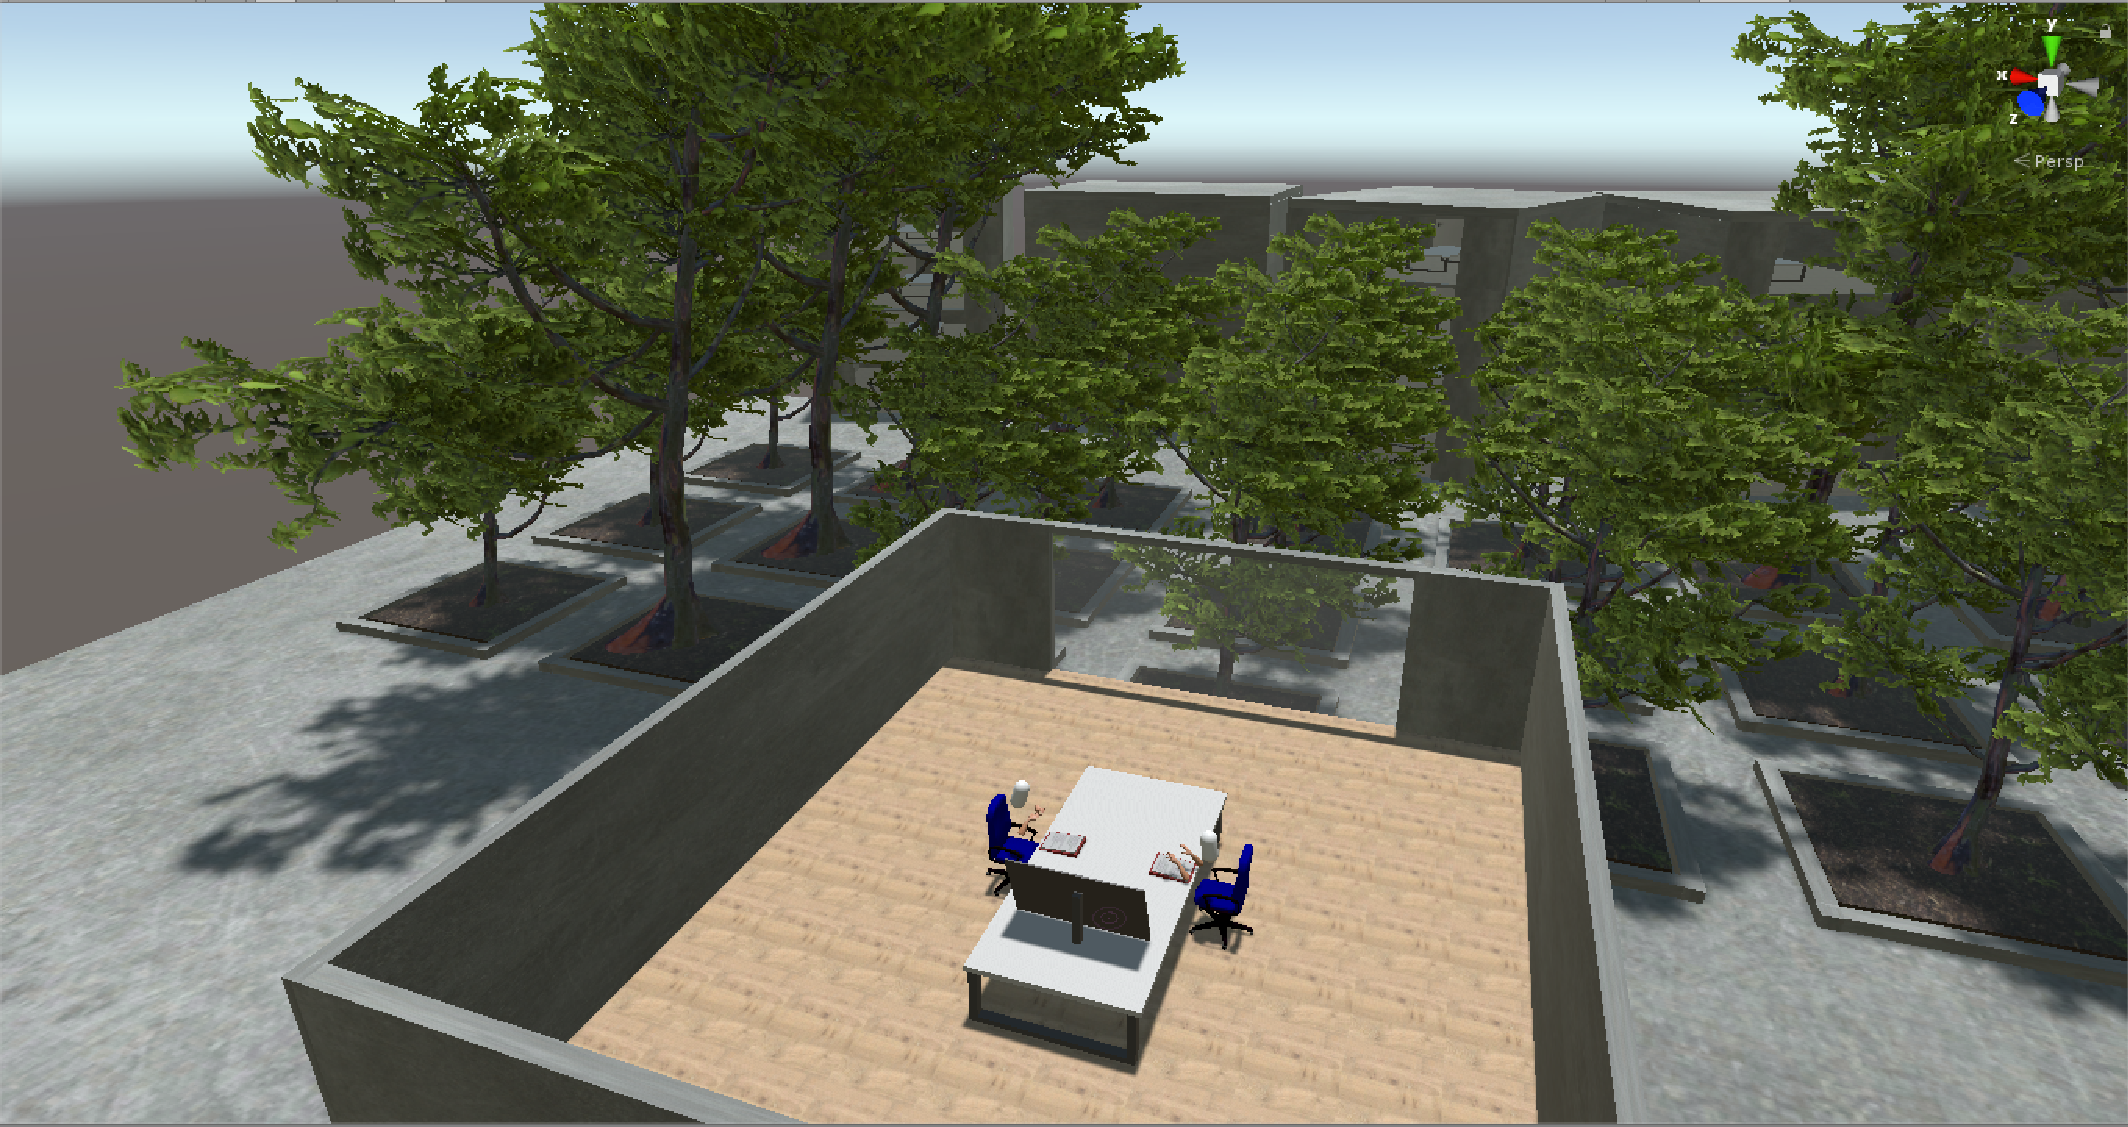
\includegraphics[width=\textwidth]{figures/far.pdf}
        \caption{Meeting room in VR.}
        \label{fig:meetingroom}
    \end{subfigure} \hfill
    \begin{subfigure}[b]{0.49\textwidth}
        \centering
        \includegraphics[width=\textwidth]{figures/nomovement.pdf}
        \caption{View in condition \textit{no movement}.}
        \label{fig:meetingroom2}
    \end{subfigure} \hfill
    \begin{subfigure}[b]{0.49\textwidth}
        \centering
        \includegraphics[width=\textwidth]{figures/benezeigtVR.pdf}
        \caption{First person view of talking participant in VR.}
        \label{fig:pointRL}
    \end{subfigure} \hfill
    \begin{subfigure}[b]{0.49\textwidth}
        \centering
        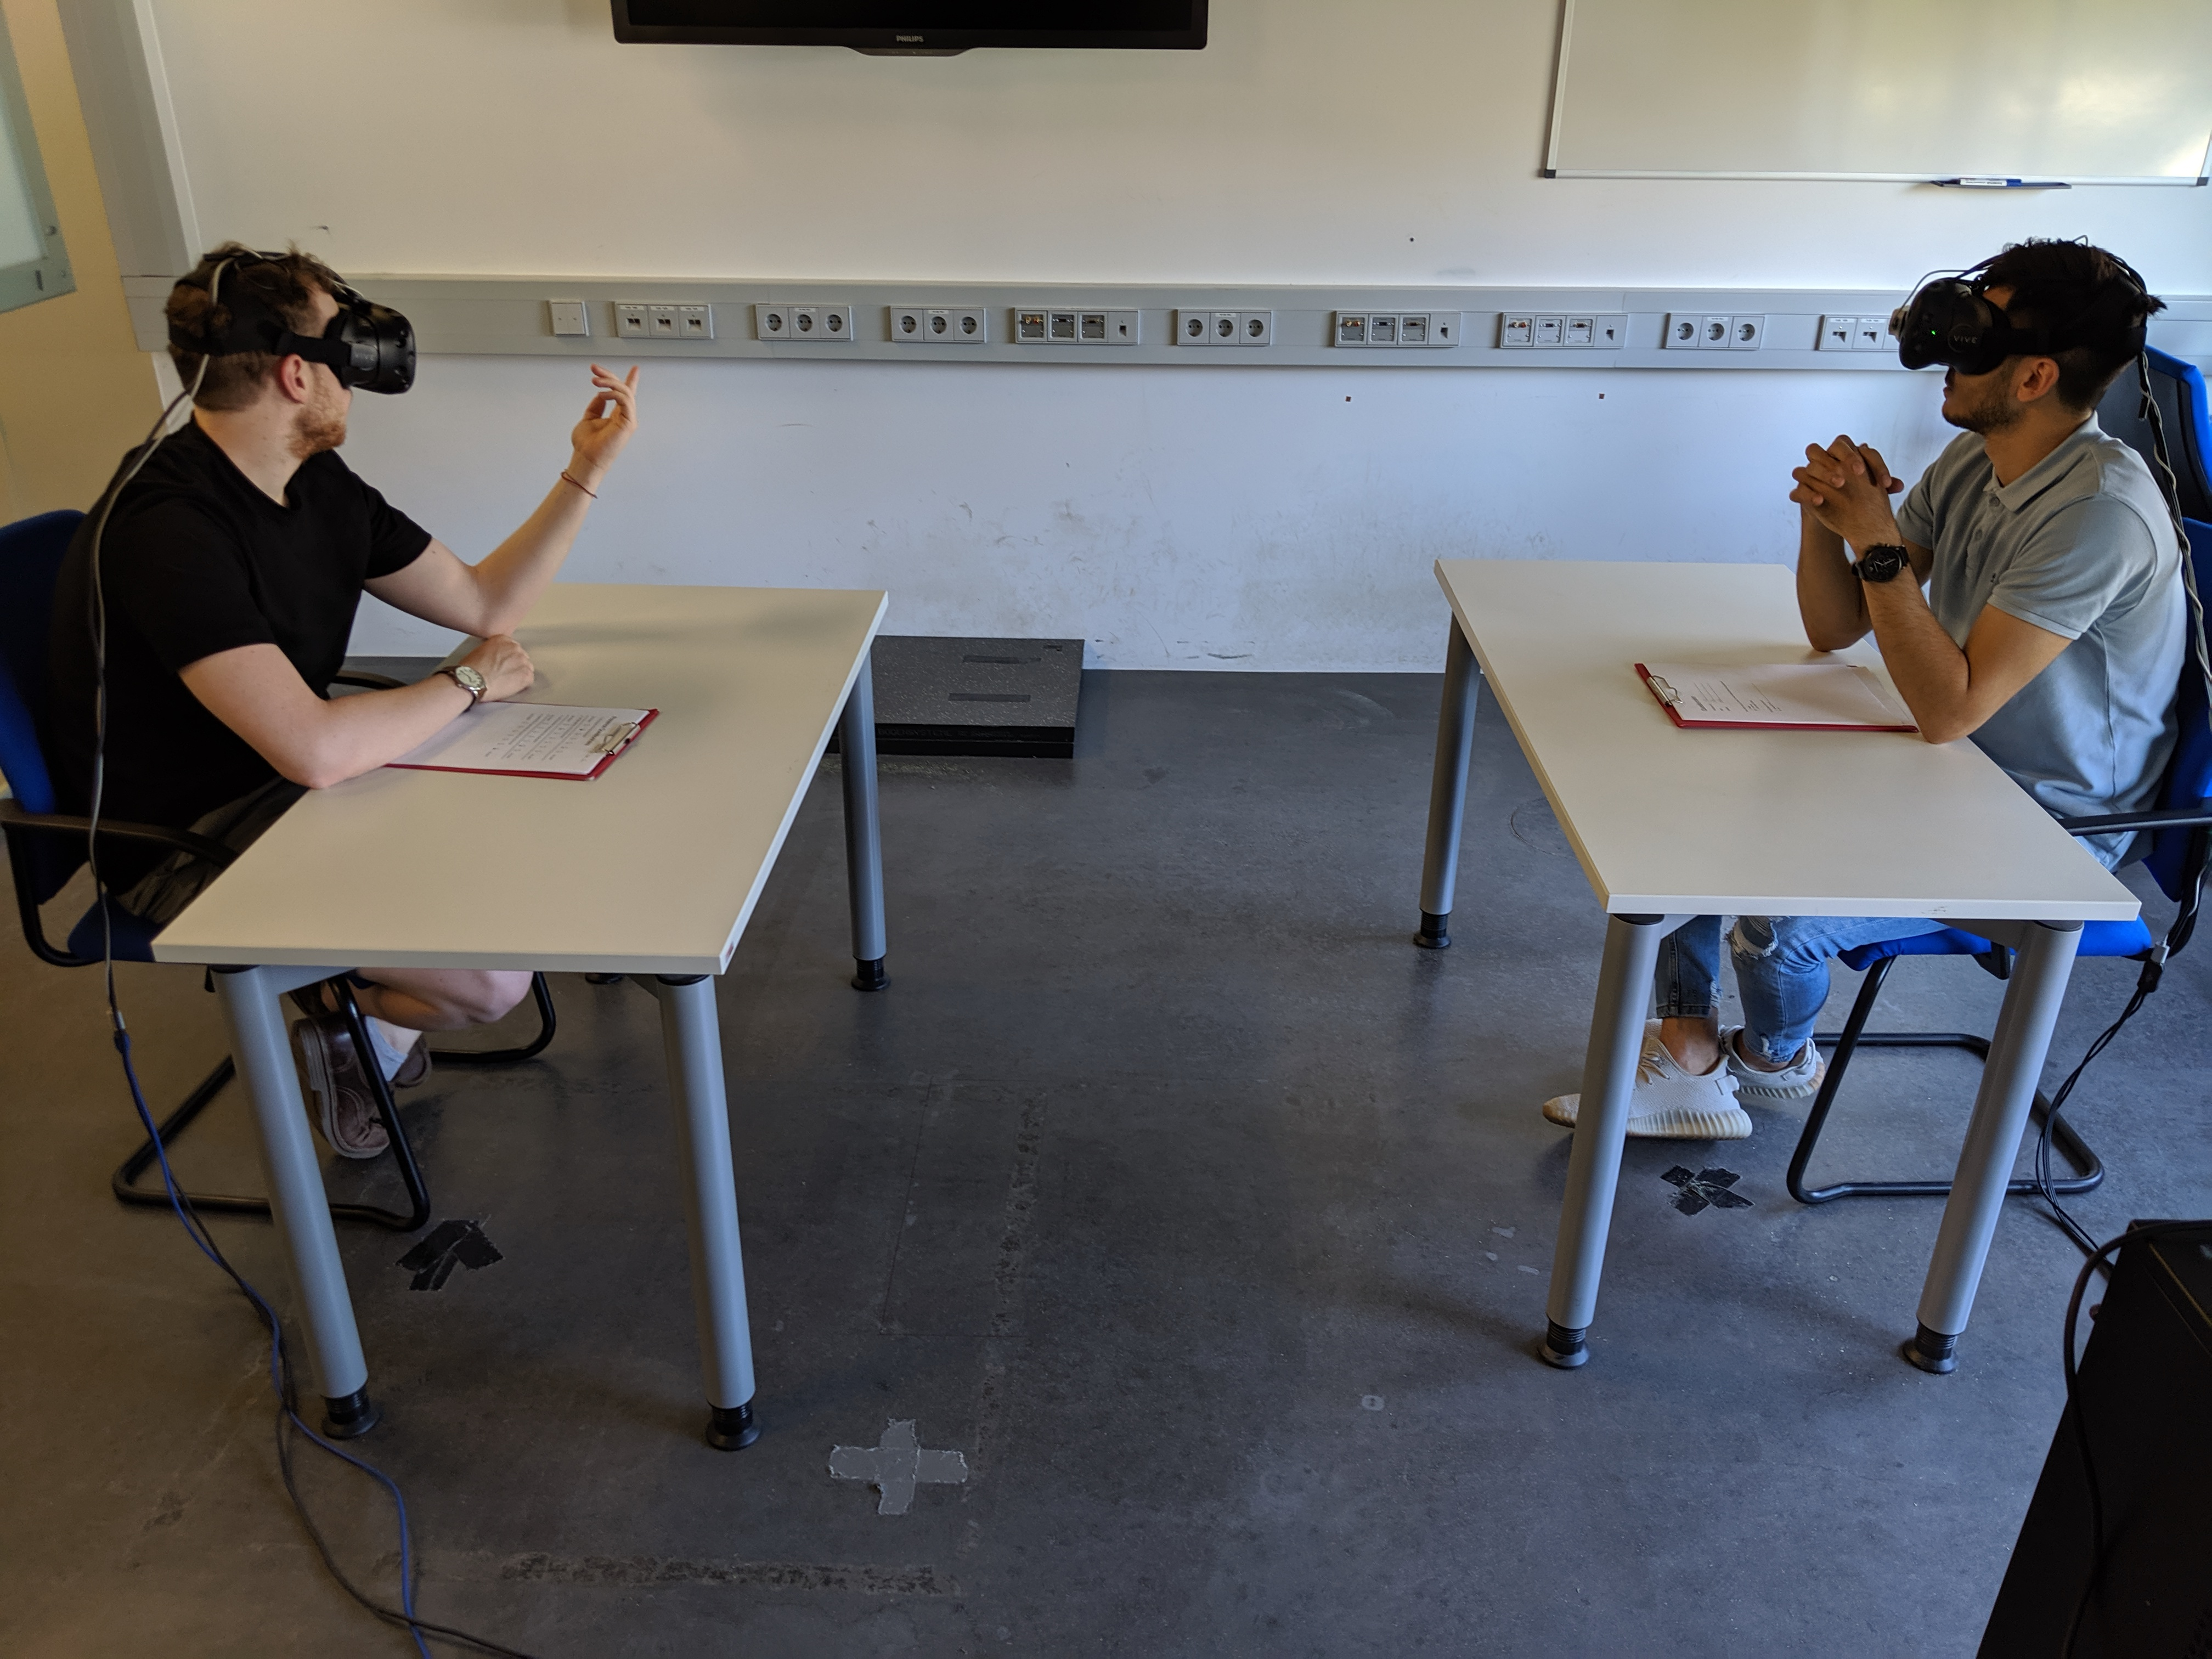
\includegraphics[width=\textwidth]{figures/benezeigtRL.pdf}
        \caption{Both participants talking in the study room. }
        \label{fig:pointVR}
    \end{subfigure}
    \caption{Pictures showing the study setup and what the participants see in VR.}
    \label{fig:studypics}
\end{figure}
\subsection{Measures}

We collected both quantitative and qualitative measurements.
The former was gathered during interviews and the latter was collected via questionnaires (subjective) and by tracking the position of the virtual palms.
This way the euclidean distance of each participants hand can be calculated. 
The questionnaires had questions from the ITQ by \citet{Witmer1998b} and questions about co-presence from \citet{poeschl2015measuring} and were handed out after every condition.
With these questionnaires we can measure presence and co-presence for each condition (see \Cref{tab:anova_presence}). 

\subsection{Procedure}
The procedure is illustrated in \Cref{fig:procedure}.
After welcoming the participants, we asked them to take a seat at two opposing tables in the same room, facing each other. 
We answered possible questions and the participants signed an informed consent from. 
As a next step, we asked them to fill in a demographics questionnaire and explained the procedure of the study. 
We told them to discuss topics which were displayed inside the virtual world without mentioning the difference between the conditions. 
We did not tell them that it was about the hand movements, but emphasised that a lively discussion was desirable. \\ \linebreak
Then, both participants put on the HMD and they had a few moments to try out how to use their hands in the virtual space. 
The study was divided into three sections, one for each condition. 
We used a Latin square to balance the order of the conditions. 
After each session, the participants filled out two questionnaires about presence and co-presence. 
When the participants had nothing more to say to the current topic, we provided new pictures and questions for them to discuss about. 
After the last session, we conducted a semi-structured interview with each participant separately. 
We then thanked the participants and answered any remaining questions. 

\begin{figure}[t]
    \centering
    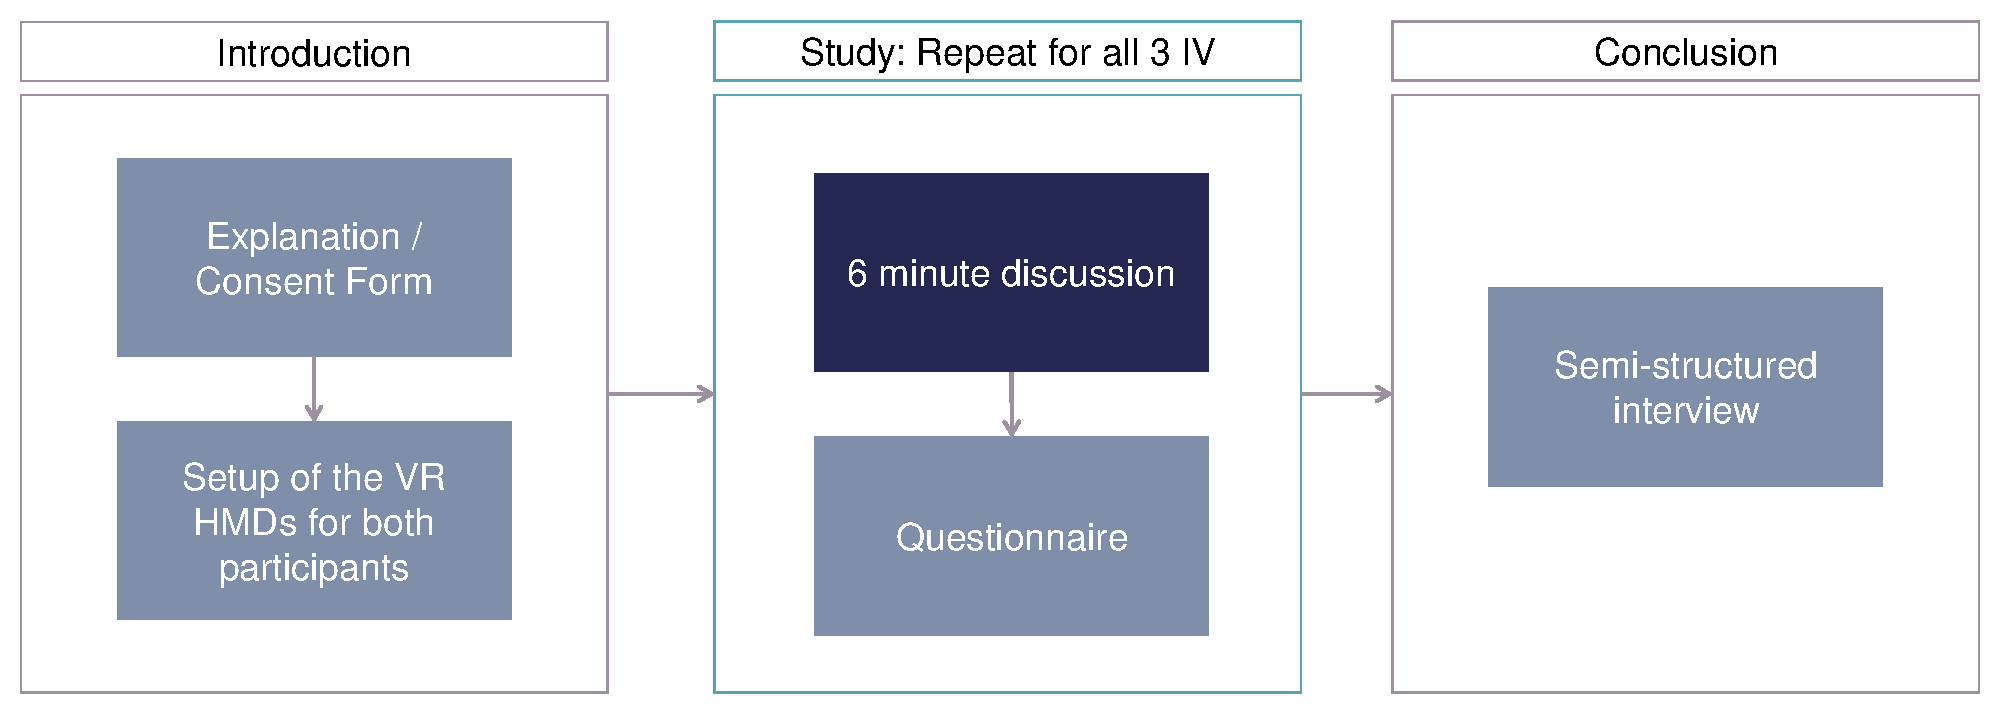
\includegraphics[width=\linewidth]{figures/procedure.pdf}
    \caption{Procedure of the study.}
    \label{fig:procedure}
\end{figure}


\subsection{Participants}
We recruited students from our university, which participated voluntarily and did not receive any compensation. 
The 12 participants (11 males, 1 female) were between 23 and 28 years old $(M = 24.5, SD = 1.51)$. We gave each participant a unique ID, ranging from 11/12 to 61/62.
Eleven of the participants had previous VR experience and only one stated to have never been in VR before.
The study lasted approximately 30 minutes, with each condition lasting 6 minutes and 42 seconds in average.

\section{Results}
\label{sec:results}
The following section contains all results of the study. 
These can be divided into two different subsections, one about the qualitative results, which includes the interviews and the second subsection describes the quantitative results, consisting of the analysis of both questionnaires and the measured distance participants covered with their hands. 

\begin{table}[tb]
    \centering
    \caption{Results of ANOVA on Aligned Rank Transformed Data of both Questionnaires.}
    
    \begin{tabularx}{\textwidth}{c@{\hskip 0.3cm} X@{\hskip 0.5cm} S[round-mode=places,round-precision=3] S[round-mode=places,round-precision=3]}
        \toprule 
        & Question & \text{F(2,22)} & p \\
        \midrule
        Q1 & I was not aware of my real environment  & 1.4648 & 0.253 \\
        Q2 & I still paid attention to the real environment  & 1.0878 & 0.35441 \\
        Q3 & I had the sensation to feel present in the virtual space &  0.30608 &  0.73941  \\
        Q4 & It seemed like my own hands were located in the virtual world &  1.3418 &  0.28195  \\
        Q5 & The others person's behaviour influences my feeling. & 1.5622 & 0.23207\\
        Q6 & The person's behaviour had an influence on my mood.  & 3.9849 & 0.033352 \\
        Q7 & I react to the other person's behaviour.& 2.374& 0.11653 \\
        Q8 & I was distracted by the other person.&3.3615 & 0.053225\\
        Q9 & Sometimes the person was influenced by my mood.& 0.39434& 0.67879 \\
        Q10 & Sometimes the person was influenced by my presence.& 1.6576& 0.21353 \\
        Q11 & The person reacted to my actions. &1.0793 &0.35717 \\
        Q12 & I was able to interpret the person's reactions. &7.4196 & 0.0034454\\
        Q13 & I had the feeling to interact with the other person. & 3.1846&0.061 \\
        Q14 & I felt connected to the other person.  &1.9856 & 0.16116 \\
        Q15 & I had the feeling that I was able to interact with the other person in the virtual space. & 0.82568& 0.45106\\
        Q16 & I had the impression that the person noticed me in the virtual space. &5.3973 &0.012383 \\
        Q17 & I was aware that other people were with me in the virtual room. &3.6286 &0.04346 \\
        Q18 & I had the feeling that I perceived the other person in the virtual room. & 0.10543& 0.90039\\
        Q19 & I felt alone in the virtual environment.  & 6.941 & 0.0046025 \\
        Q20 & The other person's movements looked awkward. &3.0862 & 0.065853\\
        Q21 & The other person was able to interact correctly. &2.1623  &0.13889 \\
        Q22 & The other person's movement seemed hindered.& 4.22   & 0.028102 \\
        \bottomrule
    \end{tabularx}
    \label{tab:anova_presence}
\end{table}

\subsection{Qualitative Results}
%Immer sagen welcher participant was gesagt hat
As mentioned above, we conducted interviews with each participant after the study to collect qualitative data about how they felt during the different conditions. 
To analyse these interviews, we transcribed the answers of all participants and then constructed an affinity diagram to cluster related statements.  \\ \linebreak
The first question concerned the general feeling of the participants during the whole study.
Most participants liked the ability to move their hands, but criticised the technical implementation. 
This concerned the artefacts of the transmission problems as described in \Cref{sec:techdifc}.
The number of participants who enjoyed the setup was balanced with the not so satisfied people. 
Most of them disliked the fact that their hands disappeared during the study due to tracking problems (see \Cref{sec:techdifc}).
Next, we asked the participants in which condition they felt most immersed. 
At this point, some of them already figured out what the difference of the conditions was, however the majority did not yet notice this. 
Most of them rated the condition with \textit{real movement} as the most immersive one, followed by the condition \textit{no movement}. 
P51 said the condition ``where the hands move the way they do in real life, and for the other person as well, feels most natural.''\\ \linebreak
The next two questions addressed the topic of whether participants find gestures important for conversations in general and whether they feel like they perform a lot of gestures themselves. 
The vast majority of people thought gestures were important, especially when it comes to discussions.
In contrast, only half of the participants said that they use many gestures during conversations. 
We also asked the participants, if they noticed the other person moving their arms. 
This was answered in favour by almost all of them, only very few stated that they noticed it subconsciously and that they were not sure if the other person moved their arms or if it was caused by tracking problems. 
We asked the participants, if the other person expressed themselves through hand movement and only one third answered yes, whereas half of the remaining people did explicitly negate this.
The other half found the movements strange and therefore said that the other person only used hand movements to express themselves every now and then. \\ \linebreak
As a conclusion, we explained the difference between the conditions to the participants, to which many responded with surprise.
\subsection{Quantitative Results} 
The results for both questionnaires can be seen in \Cref{tab:anova_presence}.
To determine if \textsc{hand movement} had a significant influence on how much presence and co-presence participants felt in the virtual space we conducted a one-way within subject repeated measures analysis of variance (RM-ANOVA).
Before performing the ANOVA, we checked if the data is normally distributed. 
The quantile-quantile plots showed a rough normal distribution. 
To conduct the RM-ANOVA, we applied the Aligned Rank Transform (ART) \footnote{\href{http://depts.washington.edu/madlab/proj/art/}{http://depts.washington.edu/madlab/proj/art/}} procedure to the feasible RATINGs, using the ARTool toolkit3 to align and rank our data of the questionnaires. 
\begin{figure}[!h]
    \centering
    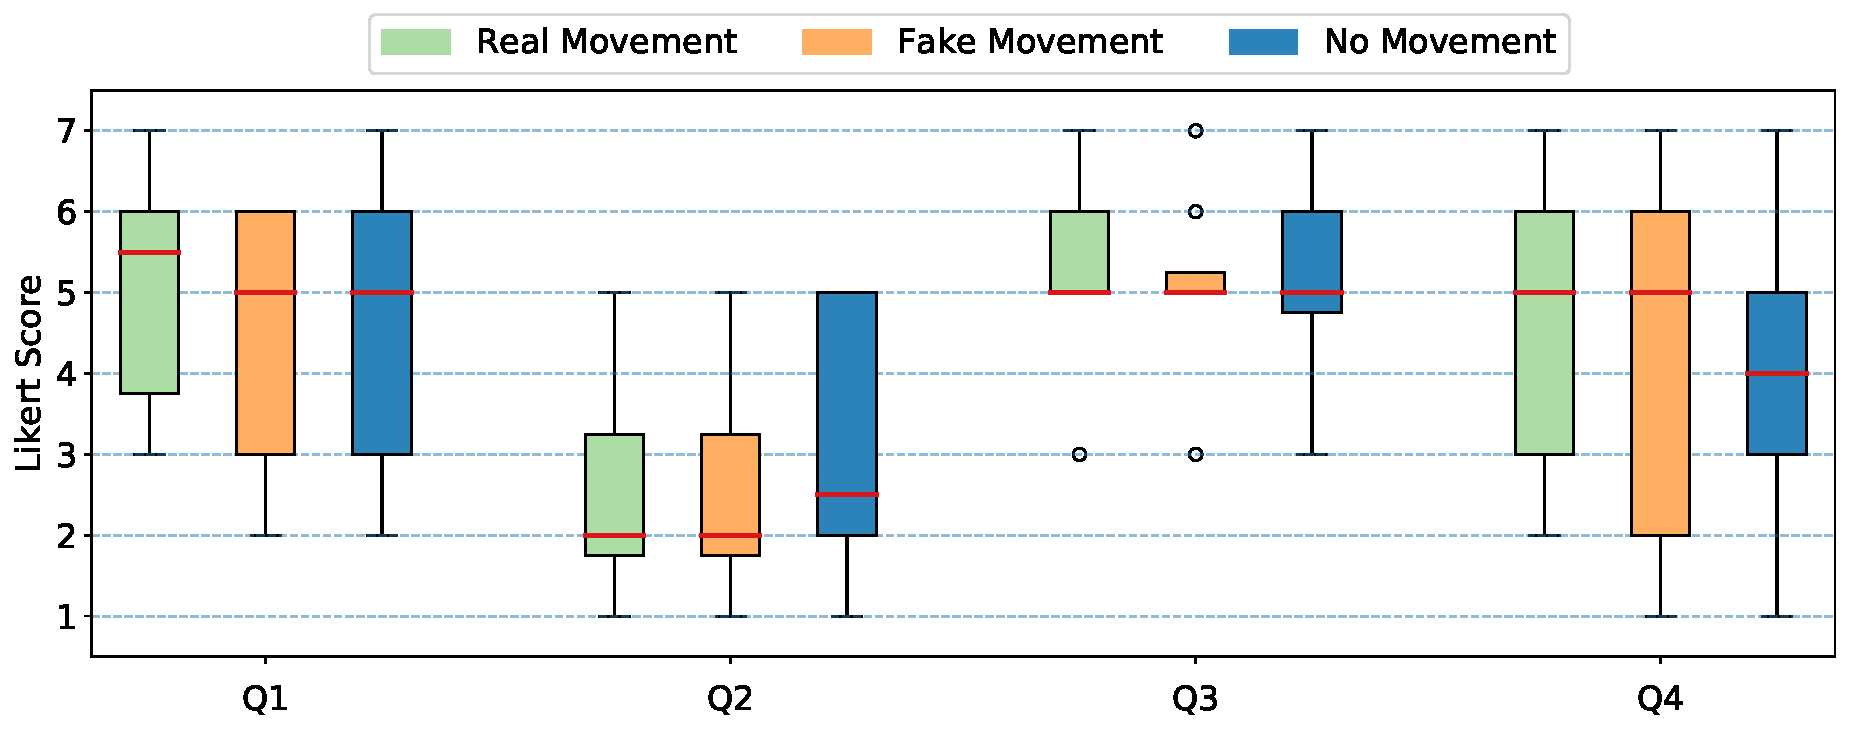
\includegraphics[width=\textwidth]{figures/presence.pdf}
    \caption{Analysis of the presence questionnaire.}
    \label{fig:presence}
\end{figure}
\begin{figure}[!ht]
    \centering
    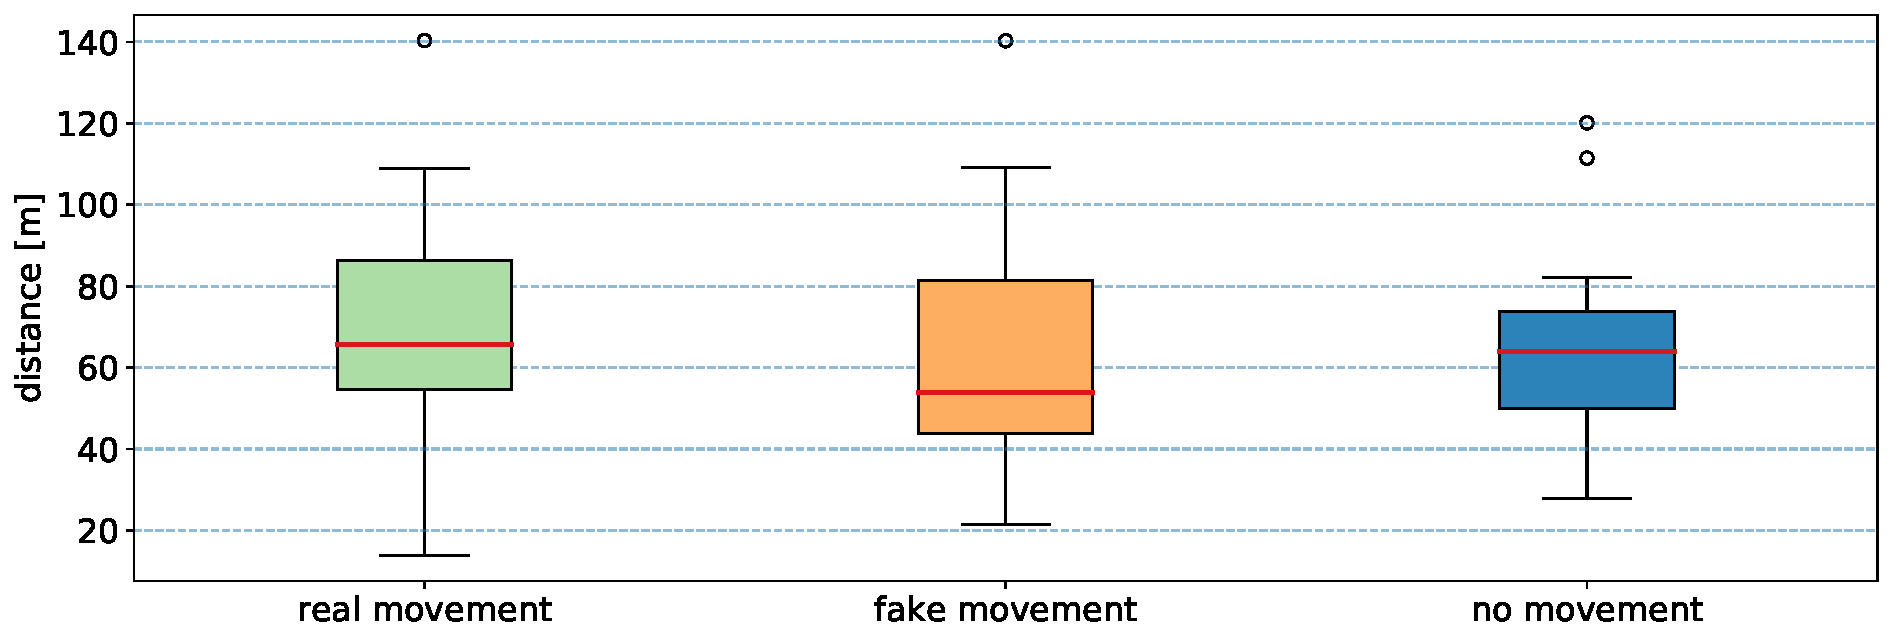
\includegraphics[width=\textwidth]{figures/euclideandistance.pdf}
    \caption{Box plots showing distance of \textsc{hand movement} in each condition.}
    \label{fig:distance_plots}
\end{figure}


\subsubsection{Questionnaire 1: Presence}
We found no significant effect on any questions and all results are listed in \Cref{tab:anova_presence}, where Q1 - Q4 are the questions about one's own felt presence.
\Cref{fig:presence} shows plots of the results for this questionnaire. 
\subsubsection{Questionnaire 2: Co-Presence}
The answers are illustrated in \Cref{fig:co-presence}.
We used a confidence level of 0.95 and found a significant effect on Q6 $[F(2, 22) = 3.9849, p = .033]$, Q12 $[F(2, 22) = 7.42, p = .0034]$, Q16 $[F(2, 22) = 5.397, p = .012]$, Q17 $[F(2, 22) = 3.63, p = .043]$, Q19 $[F(2, 22) = 6.94, p = .0046]$ and Q22 $[F(2, 22) = 4.22, p = .028]$.
We did not find any significant effect for the remaining questions. 
We performed post hoc comparisons by using Tukey HSD t-test on all significant questions. 
This showed a significant difference between \textit{no movement} $ \times $ \textit{real movement} for Q6 $(p = .0259)$. 
For Q12, there was a significant difference between \textit{fake movement} $\times $ \textit{real movement}  $(p = .0050)$, as well as \textit{no movement} $\times $ \textit{real movement}  $(p = .0144)$.
The test revealed a significant difference between \textit{no movement} $ \times $ \textit{real movement} for Q16 $(p = .0098)$ and Q19 $(p = .0034)$, as well. 
For Q22, there was a significant difference between \textit{fake movement} $ \times $ \textit{real movement} $(p = .0296)$.
\subsubsection{Euclidean distance}
We measured the distance the palm of the participants moved during each condition to check whether there is a difference between them.
The results are illustrated in \Cref{fig:distance_plots}.
For the condition \textit{real movement}, the mean distance was 71.27\,m, for the condition \textit{no movement} the mean distance was 64.52\,m and the mean value for the last condition, \textit{fake movement} was 67.67\,m.
We performed a one-way ANOVA on the data, which revealed no significant effect of the condition on the movement $[F(1, 34) = .084, p = 0.774]$.
\begin{figure}[!h] 
    \centering
    \begin{subfigure}{\textwidth} \hfill
        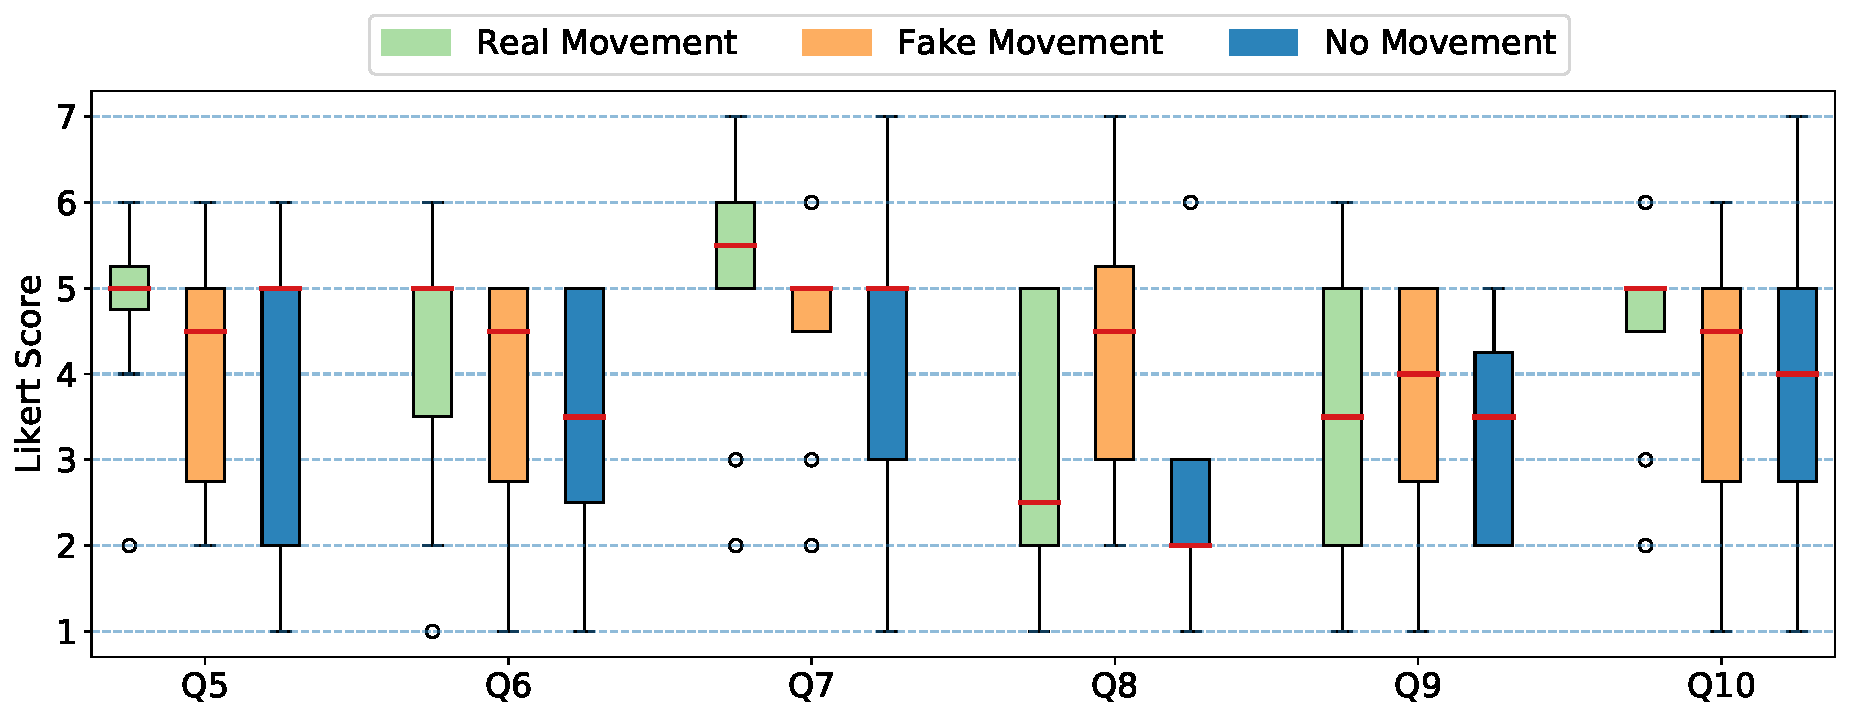
\includegraphics[width=\textwidth]{figures/co-presenceAll0.pdf}
    \end{subfigure}
     \begin{subfigure}{\textwidth} \hfill
        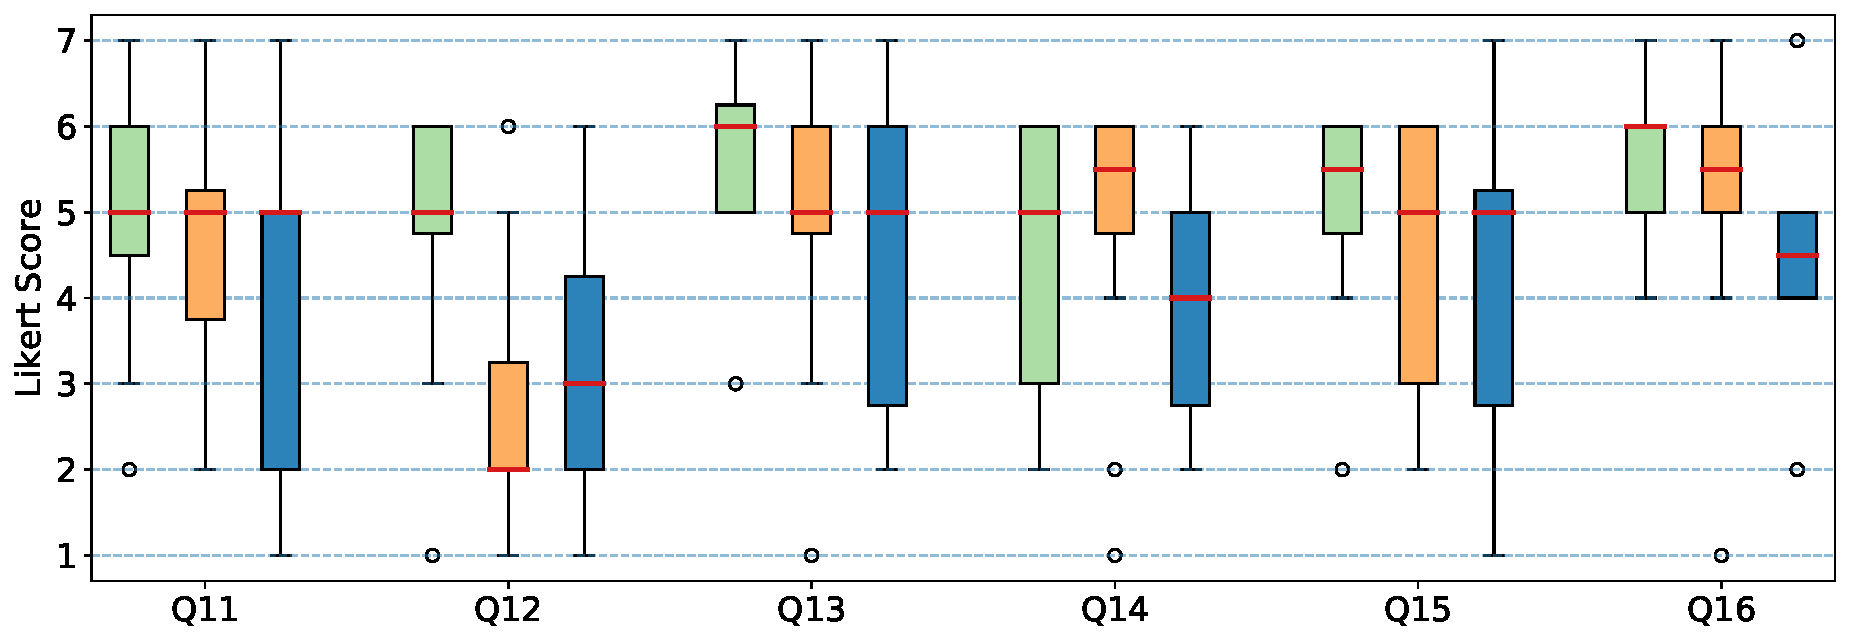
\includegraphics[width=\textwidth]{figures/co-presenceAll1.pdf}
    \end{subfigure}
     \begin{subfigure}{\textwidth} \hfill
        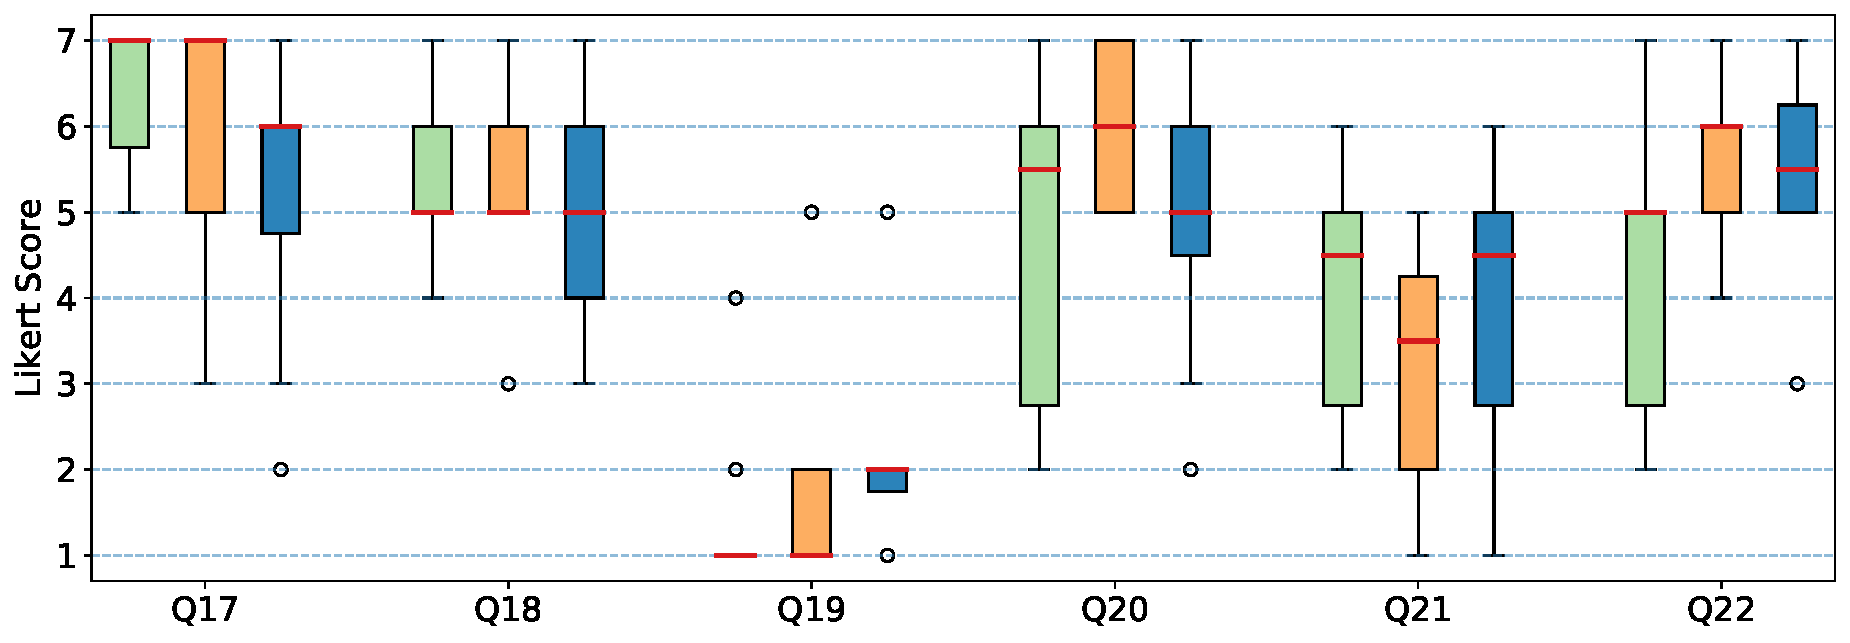
\includegraphics[width=\textwidth]{figures/co-presenceAll2.pdf}
    \end{subfigure}
    \caption{Box plots showing answers of the co-presence questionnaire.}
    \label{fig:co-presence}
\end{figure}
\newpage
\section{Report}
\label{sec:report}
In this section, the remaining questions from the milestone, which have not been answered in the paper, will be discussed. 

\subsection{Differences to Original Plan}
\label{subsec:diff}
One thing, we already described in a previous milestone submission was, that instead of using a full-body virtual avatar, we decided to only use hands and an abstract head. 
We made this decision because of two factors. 
\begin{enumerate}
    \item The workload to develop inverse kinematics for a full avatar from only the hands and head position would be way out of scope for this project.
    \item As we want to study if hand movement affects co-presence, it makes sense to shift the focus of the participants on the hands. Also as described in \cref{subsec:copre}, related work found that having a virtual avatar for talking exercises in a virtual environment, without mouth movement, is uncanny.
\end{enumerate}

\subsection{Feedback}
One group stated, that we did not have a ceiling, which could negatively influence immersion. 
\citet{slater_influence} explained that shadows also influence depth perception and thus one's presence. 
We could have placed some lamps, but the lightning with many light sources did not seem very realistic. 
As a compromise, a glass ceiling was built into our setup.

\subsection{Limitations}
Our biggest limitation for this study was using Leap motions in combination with our study setup.
As the Leap motion is a camera-based tracking system, the hands only get tracked if they are in the field of view of the camera.
However, when the participants looked at the TV-panel and did not fully turn their body, but only their head, the hands were often not tracked. 
This also sometimes occurred, when participants placed their hands on the table but looked at the other participants. 
As a result, most of the time no hands were displayed during the condition with \textit{real movement}.
This could be solved for example with tracking gloves that do not rely on seeing the hands to track. 
When the Leap motion did not track any hands, they were not rendered in the virtual environment.
This led to the undesirable effect, that for some participants, the hands of the other person were not rendered most of the time, which probably negatively influenced the feeling of presence.

\subsection{Technical Challenges}
\label{sec:techdifc}
A technical challenge was the transmission of the hands over the network. 
As each hand has 26 bones. If one bone changes the position, only this bone gets transmitted to the other computer. The amount of packages that need to be transmitted is high when participants moved their hands very fast. This led to the transferred hands looking weird at sometimes, as the position of the bones sometimes were too far away from each other.
This problem can be seen in \Cref{fig:techdifc}. \\ \linebreak
This is due to the university-network, where no UDP-traffic is allowed. Therefore, we had to use TCP, which is much slower while transmitting but ensures the other computer is receiving the packages. We also tried setting our own server up, but this did not lead to huge improvements. Another improvement could be transmitting an array with all the bones for one change. There would be a lot fewer packets to be transmitted. Then the hand could be interpolated between the new position and the one before. The advantage would be that the hand would not look unnatural at any time, because the bones remain their structure.
\begin{figure}[t]
    \centering
    \begin{subfigure}{.49\textwidth}
        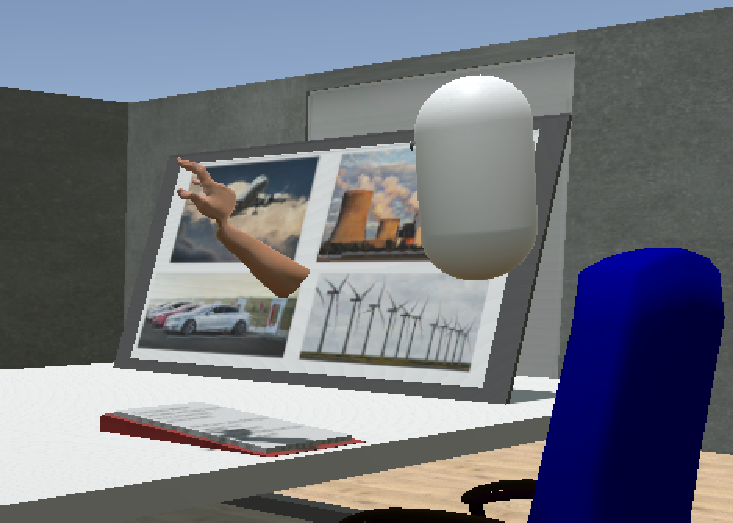
\includegraphics[width=\textwidth]{figures/techdifc.pdf}
    \end{subfigure} \hfill
     \begin{subfigure}{.49\textwidth}
        \includegraphics[width=\textwidth]{figures/techdifc3.pdf}
    \end{subfigure}
    \caption{Screenshots showing the transmission problem in VR.}
    \label{fig:techdifc}
\end{figure}

\subsection{Non-Technical Challenges}
As already shortly mentioned in \cref{subsec:diff}, we had to think about how we wanted to display the virtual avatars. 
After looking at some previous work, and gathering feedback, we decided on only rendering the human hands and a capsule as the head. 
This way the avatar is abstract enough, to not be uncanny.
Also, the focus on the study is set on hand movement.

\subsection{Features}
In this project, we build a VR application, with which it is possible to place multiple people in a virtual environment, and tracking and transferring their hand movement. 
For our project we used this, to study the effect of \textsc{hand movement} on the co-presence, but in theory, this can also be used for other multiplayer VR applications, in which hand movement is important. \\ \linebreak
More specific features for our study are the TV-panel for showing pictures and being able to iterate through them, iterating through the three conditions, and having a virtual environment representing a meeting room. \\ \linebreak
We also optimized lightning and shadows by setting up four shadow cascades\footnote{\url{https://docs.unity3d.com/Manual/DirLightShadows.html}}. 
This way shadows are rendered without a lot of aliasing effects.

\subsection{What would we have done differently?}
For the tracking, we used the Leap motion-Sensor. 
During the study, participants did not look at their hands all the time. 
As a result, the tracking of the hands was temporarily lost. In the Future a Manus/Sense Gloves could be used, so the tracking is always there.

\subsection{Advice}
Before doing a project, which involves conducting a study, either have experience of how to do so or talk to people who have experience in conduction studies. 
Then search for related work and plan the study carefully, otherwise, a lot of work is put into the implementation and parts that might be discarded.
After planning, finishing the implementation should be the main priority, because unseen problems could occur.
Often it needs more time than expected. 
The time gained here can be used to conduct more participants, and therefore get a more accurate result.

\subsection{Rating of Project}
Generally, we would rate the outcome of this project as positive. 
We found significant effects for co-presence for 6 out of 18 questions and also that users generally prefer talking to another person while seeing their hands.
We also found that participants were able to recognize the abstract avatar as a person. \\ \linebreak
Time-wise our VR application was ready for our study a little later than we expected, but as we planned a lot more time for the evaluation then needed, this was not a problem.

\subsection{Potential Directions}
Potential direction can be derived from the following discussion, but in short: \textsc{hand movement} does not affect ones' presence but in parts on the co-presence.
The problem of an unfitting tracking solution could be a key factor in getting even better results, also having more participants will be helpful for a more in-depth statistical analysis.
One big finding from this study is, that the owner felt presence does not change for the different conditions we tested. 
In contrast to the findings of \citet{staahl1999meetings}, who conducted that missing mimic harms conversations in VR, as participants were in doubt if the things they said were noticed by the other person.
\textsc{Hand movement} seems to not have the same effect, at least from the findings of our study.
Co-presence is affected by another person's hand movement.
In our study, we only found significant effects for our three conditions for 6 out of 18 questions, but in our discussion, we talk about why we think, that these results still indicate an influence on the co-presence. \\ \linebreak
As the goal of this study is to improve a VR-meeting, a future study should implement a VR environment for more than two people.
This study also should use a tracking system, which is not the leap motion, as not seeing any hands, coming from the leap motion not seeing them, resulted in negative feedback from the participants. 

\section{Discussion and Conclusion} \label{sec:discussion}
In this work we studied the effect of \textsc{hand movement} on the presence and co-presence of users in a cooperative VR-environment.
For this, we conducted a study with 6 $\times$ 2 participants, who we let have a discussion inside VR.
We used the three conditions \textit{no movement, fake movement} and \textit{real movement}.

\subsection{Presence}
Our results show that one's own presence is not affected by these different conditions, as we found no significant effects between any conditions for the presence questionnaire. 
This is supported by the amount of hand movement, participants performed for the different conditions, which we measured and calculated the Euclidean distance.
For none of the conditions, participants performed significantly less or more hand movement. 
While the \textsc{hand movement} of the other person differed, one's own hand movement was always real.
We already knew that hand movement has a positive effect on self-location and presence, but from this, we can learn, that this presence is not disturbed by another person in VR, represented by an abstract avatar, with only hands and head rendered. 
Previous work found, that a fully rendered avatar, but without mouth movement when participants talked created an uncanny feeling for the participants, which could have been an indicator, that any missing body movements can influence presence.  
But our study suggests that this is not the case for missing hand movement. 
From these two results, we can conclude, that presence seems to not be affected by the three different stages of hand movement we studied. \\ \linebreak
In the interview we conducted at the end of the study most participants even stated that they did not even notice the different conditions. 
One participant (PID 41) for instance reacted surprised and asked ``there were three different conditions? Really?''. 
After we explained the different conditions, some participants stated that they preferred seeing any kind of hands, as, for some participants who did not actively put their hands in the field of view of the leap motion, hands did not get rendered for most of the time. 
To solve this issue, a glove-based tracking system would be useful, since participants could then look in different directions other than their hands without them disappearing. 
Especially for settings with more than two people, this is mandatory, as the direction where someone looks at will often times change. 
We did not have more than two people interact with each other, but a TV-panel as a neutral third object, at which participants looked and sometimes also pointed at.
For some participants, where tracking worked, they liked the fact that the other person could express themselves with their hand movement. 
Two participants (P51 and P52) discussed environment-friendly packaging of soaps and one participant explained the shape of the soap with his hands in order to better explain to the other how solid soap looks like. 
In the interview, the listener (P52) confirmed that this helped when we asked him if the other person expressed himself through hand movements: ''Yes, especially when he talked about this soap, he showed me what it would look like and this helped me to picture it. He sometimes pointed at the board, as well. ``.
Although this did not affect our quantitative measurements regarding presence, the subjective feeling of participants seemed to be positively influenced by this. 

\subsection{Co-Presence}
In the questionnaire regarding co-presence, we found significant effects for 6 of the 18 questions.
These questions can be grouped into two categories: (1) What do I think about the other person? and (2) What does the other person think of me?
\subsubsection{What do I think about the other person?}
In the previous section, we concluded, that the own presence is not affected by the different conditions of \textsc{hand movement}, but by analyzing the qualitative measures, we found that people liked the form of expression some people had with their \textit{real movement} in VR.
Q22 is concerned with if the other persons' movement seemed to be hindered. 
We found a significant effect between \textit{real movement} $\times$ \textit{fake movement}.
To be able to read the other person's expressions, the other person has to be able to express themselves freely.
In the interview, we asked the questions if participants generally feel gesture is important in the real world and if they are doing a lot of gestures themselves. 
Almost all participants said they think hand movement is a key factor for good expression. 
From this question, we can conclude that expression in VR is not only any form of \textsc{hand movement}, as in the recorded animation in the \textit{fake movement} condition, but the participants preferred the \textit{real movement}. \\ \linebreak
Q19 asked if the participant felt alone in the virtual environment.
We found a significant effect between \textit{no movement} $\times$ \textit{real movement}.
In the \textit{no movement} condition the hands were rendered at a static position and no movement happened at all for the other persons' hands.
The median answer for this question is at ``strongly disagree''.
So for the \textit{real movement} condition participants did not have the feeling of being alone in the virtual space whatsoever. 
This is supported by Q17, if the participant was aware that other people were with him in the virtual room, where the median lies at ``strongly agree''.
Although the answers for both of the other conditions are not a complete contrast, the significant effect still shows, that \textit{real movement} affects this feeling of being not alone positively. \\ \linebreak
From this, we can conclude, that \textit{real movement} positively influences ones' own thoughts about the expressions of other people in VR and also decreases the feeling of being alone. 

%Frage 3:The other person's movement seemed hindered. 
%Frage 6: I felt alone in the virtual environment.
%Frage 5:I was aware that other people were with me in the virtual room. 


\subsubsection{What does the other person think of me?}
As a conversation always has to have two or more people, and people generally care what other people think about them, this is also an important topic to focus on in VR conversations. 
Q16 was about the impression that the other person noticed the participant in the virtual space.
If ones' own actions do not seem to have any form of effect, which is answered by a reaction by the other person, it is hard to know if the other person even understood what was said.
In the real world, this is usually done by reading the mimic of ones' conversation partner. 
\citet{staahl1999meetings} found that this missing mimic had a negative influence in VR.
We abstracted the VR avatars and thus the only form of visually reacting to the other person is hand movement, and \textit{real movement} amplified the feeling of being noticed in VR, we can state that this has a positive effect in contrast to having \textit{no movement}.
On the other hand, Q6 asked if the other person's behaviour had an influence on the participants' mood.
Again we found a significant effect between \textit{no movement} $\times$ \textit{real movement}.
So not only does \textit{real movement} positively affect the feeling of being noticed but receiving no visual reaction in a conversation in the \textit{no movement} condition even influences one's own mood.
Visually reacting to the other person and also expressing oneself is key for conversations in the real world.
Not being able to do this seemed strange to the participants. 
Some participants even stated during the study ``Are you not moving your hands?'' while being in the \textit{no movement} condition. \\ \linebreak
We found, that the different conditions had no effect on one's own presence.
But we found that being able to express oneself and reading the other person's expression amplifies the feeling of not being alone, being noticed, and even has an effect on the own mood.
In the \textit{fake movement} condition expressions were given as random moving animations, but the results from Q12, which asked the participants if they were able to interpret the person's reactions, show that \textit{real movement} outperforms not only \textit{no movement} but also \textit{fake movement}.
So not only is it important to show any form of reaction or expression in VR but being able to express oneself the way one would do in the real world, gives participants the opportunity to even interpret these reactions.
The strong significant effect between \textit{real movement} $\times$ \textit{no movement} and \textit{fake movement} shows that being able to interpret the other persons' reaction is only possible if that person is able to correctly express themselves. \\ \linebreak
From this, we can conclude that being able to show real hand movement in VR increases the feeling of being together in a virtual space while having a conversation.
But the results only show significant effects for \textsc{hand movement} for 6 out of the 18 questions from the co-presence questionnaire.
Although this shows, that hand movement has some form of effect on the co-presence, we can not fully state if the co-presence if positively affected by \textsc{hand movement}.

%Frage 4:I had the impression that the person noticed me in the virtual space. 
%Frage 1:The person's behaviour had an influence on my mood. 
%Frage 2:I was able to interpret the person's reactions.


\subsection{Implications}
This study implicates that for a cooperative VR setting, where inter-human interaction is important, and an avatar is displayed in a very abstract way, hand movement does not affect their own presence.
This means that if only the own presence is important, the hand movement of other people in VR is not important.
The co-presence, on the other hand, is positively affected by real hand movement. 
So if multiple people have to interact with each other in VR, and the hands are the only form of visually reacting to other people, people prefer to visually react or express themselves with real hand movement.

\subsection{Future Work}
We have two main points for improving this work in future studies.
First using a different hand tracking method than the leap motion.
A non-camera-based tracking method would we advantageous, but also other optical tracking systems as Optitrack would be great.
The problem with the leap motion is, that hands are only tracked if the users look directly at them.
As soon as he moves the head to a different orientation the hands are not tracked anymore, and any other user in VR does not see them.
From our results, we can derive that real hand movement was better then the other conditions, but it was also stated in the interview at the end of the study by multiple participants that it was negatively affecting the interaction if no hands of the other participant at all. \\ \linebreak
The second thing, a future study should do differently is rendering a full avatar instead of only the head and the hands.
We talked in \cref{subsec:diff} about our reasoning behind only rendering the hands and the head for this study.
Thus being able to visually react to the other person was only possible with the hands.
In the real world, this is possible in multiple more ways.
What could be studied is if other options for visually expressing oneself in VR, still leads to finding expression through hand movement important and thereby increasing the co-presence? \\ \linebreak
Future studies could also scale the number of people in VR. 
Interaction between more than two people could lead to more hand gestures, and thus even more results on hand movement for co-presence.



%\subsubsection*{Acknowledgments}
%\ldots

%In the bibliography, use \texttt{\textbackslash textsuperscript} for \qq{st}, \qq{nd}, \ldots:
%E.g., \qq{The 2\textsuperscript{nd} conference on examples}.
%When you use \href{https://www.jabref.org}{JabRef}, you can use the clean up command to achieve that.
%See \url{https://help.jabref.org/en/CleanupEntries} for an overview of the cleanup functionality.

\renewcommand{\bibsection}{\section*{References}} % requried for natbib to have "References" printed and as section*, not chapter*
% Use natbib compatbile splncsnat style.
% It does provide all features of splncs03, but is developed in a clean way.
% Source: http://phaseportrait.blogspot.de/2011/02/natbib-compatible-bibtex-style-bst-file.html
\bibliographystyle{splncsnat}
\begingroup
  \ifluatex
    %try to activate if bibliography looks ugly
    %\sloppy
  \else
    \microtypecontext{expansion=sloppy}
  \fi
  \small % ensure correct font size for the bibliography
  \bibliography{VR_MeetingStudy}
\endgroup

% Enfore empty line after bibliography
\ \\
%
All links were last followed on July 5, 2019.
\end{document}
